\documentclass[UTF8]{resume}

\name{郑力铖}
\address{\faPhone~+86 189 1892 8753 \faEnvelope~\href{mailto://zhenglicheng@shu.edu.cn}{zhenglicheng@shu.edu.cn} \faGithub~\href{https://github.com/SHUzheking/}{GitHub: SHUzheking} \faWeixin~2035451658~~~~~}
\address{}

\begin{document}

\begin{tikzpicture}[remember picture, overlay] 
  \node[anchor = north east] at ($(current page.north east)+(-1.2cm,-1.2cm)$) {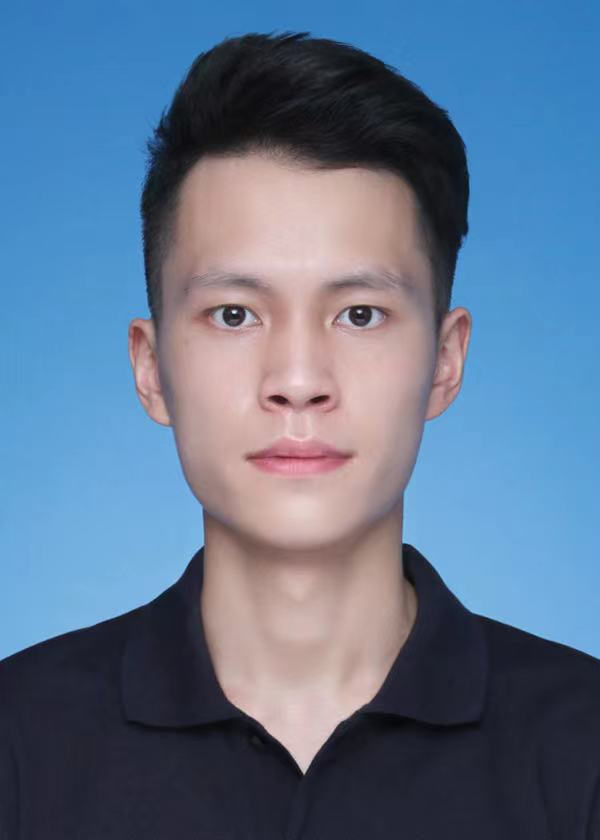
\includegraphics[height=2.5cm]{avatar.jpg}};
\end{tikzpicture}

\begin{rSection}{\faGraduationCap~教育经历}
    \begin{itemize}
        \item 上海大学~计算机工程与科学学院~人工智能系~\hfill 2021.09-今 \\ GPA~84.7/100
    \end{itemize}
\end{rSection}
 

\begin{rSection}{\faUsers~项目经历}
    \begin{rProject}{校内科研}{面向NASICON型电解质的描述符自动获取方法研究}{2022.05 - 2023.03}
        \textbf{项目概述}:利用文本挖掘方法,从小批量NASICON 型固态电解质文献中,抽取描述符并以此构建模型进行训练,实现自动、高效地获取NASICON 型固态电解质描述符。\\
        \textbf{项目开发}:使用\textbf{Vue}开发前端界面,后端开发使用\textbf{Springboot}与\textbf{MySQL}数据库进行通信。并使用\textbf{Pytorch}部署BERT算法用于论文处理,提取出的描述符使用\textbf{Neo4j}进行知识图谱的建构。\\
        \textbf{负责部分}:组员,负责前后端开发、数据库设计和管理、代码整合。有Python编写的脚本将数据发送给前端绘制。
    \end{rProject}

    \begin{rProject}{团队项目}{面向RoboMaster机器人的计算机视觉算法识别系统}{2021.10 - 2022.12}
        \textbf{项目概述}:通过部署在机器人云台上的工业相机的视频流,识别敌方机器人装甲板与能量机关,并发布目标坐标信息使云台锁定在识别中心。其效果类似于~\textit{自瞄外挂}。\\
        \textbf{项目开发}:在Ubuntu上利用\textbf{CUDA}部署yolo网络进行识别,并通过卡尔曼滤波与弹道模型,预测运动轨迹以改善弹丸落点,实现精准打击。\\
        \textbf{负责部分}:前一年时间担任组员,负责硬件管理与相机接口开发,了解CUDA部署部分代码;后半年任组长,有管理与培训经验。
    \end{rProject}
\end{rSection}

\begin{rSection}{\faAward~获奖经历}
    \begin{itemize}
        \itemsep -0.5em
        \item 第二十一届全国大学生机器人大赛RoboMaster机甲大师超级对抗赛全国赛~三等奖 \hfill 2022.08
        \item 第三十五届上海市青少年科技创新大赛~计算机科学~《基于图像识别技术识别简单乐谱并演奏》~一等奖 \hfill 2020.04
        \item 首届全球中学生人工智能交流展示会~《基于图像识别技术识别简单乐谱并演奏》~一等奖 \hfill 2019.03
        \item 上海市青少年机器人知识与实践比赛~智能驾驶项目~中学组~一等奖 \hfill 2018.11/2019.11
        \item 首届上海市青少年人工智能挑战赛~智能驾驶锦标赛~高中组~一等奖 \hfill 2018.11
    \end{itemize}
\end{rSection}


\begin{rSection}{\faCogs~编程经验}
  \begin{itemize}
      \itemsep -0.5em
      \item 编程语言(熟悉): C++、Python、HTML、CSS、MATLAB、\LaTeX; 
      \item 编程语言(了解): Vue、JavaScript、Java、SQL;
      \item 工具(熟练): Bash、Git; 
      \item 技术原理(了解): C编译原理、CUDA编程、机器学习、深度学习.
  \end{itemize} 
\end{rSection}


\end{document}